\documentclass{article}
\usepackage{amsmath}
\usepackage[margin=1in]{geometry}
\usepackage{amsfonts}
\usepackage{hyperref}
\usepackage{graphicx}
\usepackage{amssymb}

\begin{document}
	
	\title{Linear Transformations}
	\author{Andy Chong Sam}
	
	\maketitle
	
	\section{Introduction}
	
	\par\noindent To introduce this topic we start with the idea of a function. The generic function \(f(x)=y\) contains an independent variable \(x\) and a dependent variable \(y\). Assigning to \(x\) some number and using it in the function's calculation gives us a unique value \(y\). 
	\newline
	\par\noindent This concept extends to the realm of vectors. Instead of treating an individual number as an independent variable, we use an input vector. In this document we'll call this \( \vec v\). A matrix will encode the calculation being peformed. This is traditionally called matrix \(A\). The result of this operation is matrix \(B\). This is written in the form of a matrix multiplication:
	
	\begin{flalign*}
		A\vec{v} = B
	\end{flalign*} 

	\par\noindent We can also describe the environment in which this operation takes place. This is often written in the following form: 
	
		
	\begin{flalign*}
		T: \mathbb{R}^n \rightarrow \mathbb{R}^m
	\end{flalign*} 

	\par\noindent The letter \(T\) denotes that this is describing a transformation. The input vector is from the vector space \(\mathbb{R}^n\) . This space is known as the \textbf{domain}. If we have, for instance, \(\mathbb{R}^2\) we are saying that this transformation accepts a two dimensional vector with a real \(x\) and \(y\) component. Next we define what the transformation itself does. 
	\newline
	\par\noindent Here is an example, where \(T:\mathbb{R}^2 \rightarrow \mathbb{R}^2\)
	
		 \[
		T
		\left(\begin{array}{@{}c@{}}
			x \\
			y \\
		\end{array}\right) = 
			\left(\begin{array}{@{}c@{}}
		2x \\
		3y \\
	\end{array}\right) 
		\]
		
	\par\noindent In this example, feeding the transformation a two dimension vector, say \(<1,3>\) results in another two dimension vector \(<2,9>\).
	\newline
	\par\noindent It's also possible to rewrite the transformation in its standard form \(A \vec v = B\). To do this we will use the standard coordinate vectors:
	
			 \[
	e_1 =
	\left(\begin{array}{@{}c@{}}
		1 \\
		0 \\
		0 \\
		...\\
		0
	\end{array}\right),
 	e_2 =
 \left(\begin{array}{@{}c@{}}
 	0 \\
 	1 \\
 	0 \\
 	...\\
 	0
 	\end{array}\right), 
 	e_3 =
 \left(\begin{array}{@{}c@{}}
 	0 \\
 	0 \\
 	1 \\
 	...\\
 	0
 \end{array}\right)
	\]
	
	\par\noindent The number of vectors needed is the same as the dimensions of the input vector. The matrix A, which encapsulates the transformation is composed of the columns that result from \(T(e_n)\).
	\newpage
	\par\noindent We can now rewrite the following transformation:
	\[
	T
	\left(\begin{array}{@{}c@{}}
		x \\
		y \\
	\end{array}\right) = 
	\left(\begin{array}{@{}c@{}}
		2x \\
		3y \\
	\end{array}\right) 
	\]
			 \[
	T(e_1) = T
	\left(\begin{array}{@{}c@{}}
		1 \\
		0 \\
	\end{array}\right) = 
	\left(\begin{array}{@{}c@{}}
		2 \\
		0 \\
	\end{array}\right) , 
	T(e_2)=T
	\left(\begin{array}{@{}c@{}}
		0 \\
		1 \\
	\end{array}\right) = 
	\left(\begin{array}{@{}c@{}}
		0 \\
		3 \\
	\end{array}\right) 
	\]
	\newline
	\par\noindent So we get:
	\[A=
		\left(\begin{array}{@{}cc@{}}
		2 & 0 \\
		0 & 3 \\
	\end{array}\right)
	\]
	\par\noindent We can now write the transformation in its standard form:
		\[A=
	\left(\begin{array}{@{}cc@{}}
		2 & 0 \\
		0 & 3 \\
	\end{array}\right)
	\left(\begin{array}{@{}c@{}}
	x \\
	y \\
\end{array}\right) = B
	\]
		
	
\section{Image and Kernel}
\par \noindent The image is the vector space that the transformation will end up occupying. If the definition of the transformation is given, this is a trivial process. In the example we've been using:

 	\[
 T
 \left(\begin{array}{@{}c@{}}
 	x \\
 	y \\
 \end{array}\right) = 
 \left(\begin{array}{@{}c@{}}
 	2x \\
 	3y \\
 \end{array}\right) 
 \]
	
\par \noindent We can describe the \textbf{image} as: \(x=2s\) and \(y=2t\), where \(s,t \in \mathbb{R}\). Now suppose you were not given the transformation definition but only matrix A. We can arrive at the transformation by simply carrying out the matrix multiplication of the standard form:

		\[A=
\left(\begin{array}{@{}cc@{}}
	2 & 0 \\
	0 & 3 \\
\end{array}\right)
\left(\begin{array}{@{}c@{}}
	x \\
	y \\
\end{array}\right) = 
 \left(\begin{array}{@{}c@{}}
	2x \\
	3y \\
\end{array}\right) 
\]	

\par \noindent We can describe the \textbf{kernel} as the solution to \(A \vec v = \vec 0\). 
\newline
\par \noindent For the transformation we've been looking at, the only way to obtain the zero vector is if \(x=0\) and \(y=0\). We can therefore say:
\[
Ker(T) = 
\left(\begin{array}{@{}c@{}}
	0 \\
	0 \\
\end{array}\right) 
\]
\par \noindent For more complex transformations, applying row elimination can be used to formulate the kernel. Consider the following transformation:

\begin{flalign*}
T: \mathbb{R}^3 \rightarrow \mathbb{R}^2
\end{flalign*}
\[
T
\left(\begin{array}{@{}c@{}}
	x \\
	y \\
	z
\end{array}\right) = 
\left(\begin{array}{@{}c@{}}
	x -z\\
	x + 2y - 4z\\
\end{array}\right) 
\]	

\par \noindent To determine the kernel we solve for the system of equations comprised of \(x-z=0\) and \(x+2y-4z=0\). Row reduction can be used here:
\[
\left(\begin{array}{@{}ccc@{}}
1 & 0 & -1 \\
1 & 2 & -4 \\
\end{array}\right) 
\xrightarrow[]{R_2 - R_1 = R_2}
\left(\begin{array}{@{}ccc@{}}
	1 & 0 & -1 \\
	0 & 2 & -3 \\
\end{array}\right)
\xrightarrow[]{\frac{1}{2}R_2 = R_2} 
\left(\begin{array}{@{}ccc@{}}
	1 & 0 & -1 \\
	0 & 1 & -\frac{3}{2} \\
\end{array}\right)
\]	
\[
	Ker(T) = \left\{ \begin{array}{r} 
		x= s \\
		y= \frac{3}{2}s \\
		z = s
	\end{array} \right\}, s \in \mathbb{R} 
\]
The key point is that for any value of \(s\) the \(x\), \(y\), \(z\) values produced, when plugged into the transformation will always result in the zero vector.
\section{Set Visualization}
\par \noindent We can now draw a diagram that brings together all these terms:
\newline
\newline
\begin{minipage}[c]{.5\linewidth}
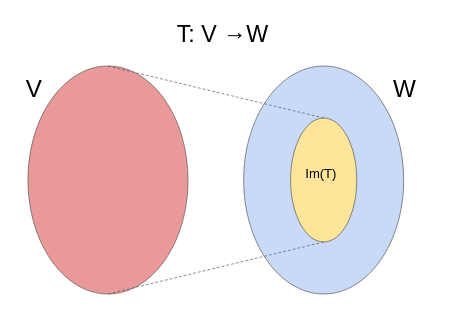
\includegraphics[width=4cm]{lt-image.png}
\newline
\textbf{Figure 1}
\end{minipage}
\begin{minipage}[c]{.5\linewidth}
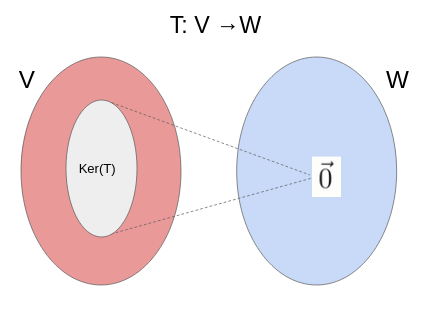
\includegraphics[width=4cm]{lt-kernel.png}
\newline
\textbf{Figure 2}
\end{minipage}
\newline
\newline
\par \noindent In figure 1, V represents the domain and W the codomain. The possible set of vectors produced by the transformation are represented by the yellow subset within W. This subset is the image of T. In figure 2, there is a subset within the domain that will always be transformed into the zero vector, thus the gray subset within V is the kernel of T.
\section{Linear Transformation}
\par \noindent Although we can use this terminology to describe all transformations, not all transformations are linear. A \textbf{linear transformation} must meet certain conditions.
\newline
\par \noindent \(T: \mathbb{R}^n \rightarrow \mathbb{R}^m\) is a linear transformation if the following conditions hold:
\begin{itemize}
	\item \(T(\vec u + \vec v) = T(\vec u) + T(\vec v)\), where \(\vec u,\vec v \in \mathbb{R}^m\)
	\item \(T(k \vec v) = k T( \vec v)\) for a scalar k.
\end{itemize}
\par \noindent Let's demonstrate that the two transformations we've examined are indeed linear transformations. Let \(\vec u=<a,b>\) and \( \vec v = <c,d>\) and \(k\) a scalar:
\newline
\newline
\begin{minipage}[c]{.5\linewidth}
		 \[
T
\left(\begin{array}{@{}c@{}}
	x \\
	y \\
\end{array}\right) = 
\left(\begin{array}{@{}c@{}}
	2x \\
	3y \\
\end{array}\right) 
\]
		 \[
T(\vec u) + T(\vec v)= 
\left(\begin{array}{@{}c@{}}
	2a \\
	3b \\
\end{array}\right) +
\left(\begin{array}{@{}c@{}}
	2c \\
	3d \\
\end{array}\right) =
\left(\begin{array}{@{}c@{}}
	2(a + c) \\
	3(b + d) \\
\end{array}\right) 
\]
		 \[
T(\vec u + \vec v) = 
\left(\begin{array}{@{}c@{}}
	2(a+c) \\
	3(b+d) \\
\end{array}\right)
\]
\par\noindent \textbf{First condition met}
\newline
 \[
 T(k \vec u)= 
 k\left(\begin{array}{@{}c@{}}
 	2a \\
 	3b \\
 \end{array}\right) =
 T(k \vec u)= 
\left(\begin{array}{@{}c@{}}
	2ak \\
	3bk \\
\end{array}\right) 
 \]

\[
	kT(\vec u) = k
	\left(\begin{array}{@{}c@{}}
		2a \\
		3b \\
	\end{array}\right) =
 \left(\begin{array}{@{}c@{}}
 	2ak \\
 	3bk \\
 \end{array}\right) 
\]
 \[
 \]
 \par\noindent \textbf{Second condition met}
 
\end{minipage}
\begin{minipage}[c]{.5\linewidth}
\[
T
\left(\begin{array}{@{}c@{}}
	x \\
	y \\
	z
\end{array}\right) = 
\left(\begin{array}{@{}c@{}}
	x -z\\
	x + 2y - 4z\\
\end{array}\right) 
\\
\]
\[
T(\vec u) + T(\vec v) = 
\left(\begin{array}{@{}c@{}}
	a-c \\
	a + 2b - 4c \\
\end{array}\right)+
\left(\begin{array}{@{}c@{}}
	d-f \\
	d + 2e - 4f \\
\end{array}\right)
\]	
\[=
\left(\begin{array}{@{}c@{}}
	a-c+d-f \\
	a + 2b - 4c + d + 2d - 4f \\
\end{array}\right)
\]
\[
T(\vec u + \vec v) = 
\left(\begin{array}{@{}c@{}}
	(a+d) - (c+f) \\
	(a+d) + 2(b-e)-4(c+f)\\
\end{array}\right)
\]
\[
=
\left(\begin{array}{@{}c@{}}
	a-c+d-f \\
	a + 2b - 4c + d + 2d - 4f \\
\end{array}\right)
\]
 \par\noindent \textbf{First condition met}
\[
T(k \vec u) = 
\left(\begin{array}{@{}c@{}}
	ak - ck \\
	ak + 2yk - 4zk \\
\end{array}\right)=
k
\left(\begin{array}{@{}c@{}}
	a - c \\
	a + 2y - 4z \\
\end{array}\right)
\]
\[
kT(\vec u) = k
\left(\begin{array}{@{}c@{}}
	a - c \\
	a + 2y - 4z \\
\end{array}\right)
\]
\par\noindent \textbf{Second condition met}	
	
\end{minipage}

\section {Additional Problems}
\framebox{
	\parbox{\linewidth}{
\par \noindent \textbf{Ex. 1}  Is the following a linear transformation?
\begin{flalign*}
	T: \mathbb{R}^2 \rightarrow \mathbb{R}^2 
\end{flalign*}
\[
T
\left(\begin{array}{@{}c@{}}
	x \\
	y \\
\end{array}\right) = 
\left(\begin{array}{@{}c@{}}
	x^2 \\
	y^2 \\
\end{array}\right)
\]
\par\noindent Let \(\vec u=<a,b>\) and \( \vec v = <c,d>\).
\newline
\par\noindent We test the first condition:
\[
T(\vec u) + T(\vec v) = 
\left(\begin{array}{@{}c@{}}
	a^2 + c^2 \\
	b^2 + d^2 \\
\end{array}\right)
\]
\[
T(\vec u + \vec v) = 
\left(\begin{array}{@{}c@{}}
	(a+c)^2 \\
	(b+d)^2 \\
\end{array}\right) = 
\left(\begin{array}{@{}c@{}}
	a^2 + 2ac + c^2 \\
	b^2 + 2bd + d^2 \\
\end{array}\right)
\]
\par \noindent Since \(T(\vec u) + T(\vec v) \ne T(\vec u + \vec v)\), \textbf{this is not a linear transformation}.
}}
\newline
\newline
\newline
\framebox{
	\parbox{\linewidth}{
\textbf{Ex. 2}	Is the following a linear transformation?
\begin{flalign*}
	T: \mathbb{R}^3 \rightarrow \mathbb{R}^4
\end{flalign*}
\[T
\left(\begin{array}{@{}c@{}}
	x \\
	y \\
	z \\
\end{array}\right) = 
\left(\begin{array}{@{}c@{}}
	x + y\\
	y + z \\
	x - z \\
	z - y
\end{array}\right)
\]
\par\noindent Let \(\vec u=<a,b>\) and \( \vec v = <c,d>\).
\newline
\par\noindent We test the first condition:	
\[
T(\vec u) + T(\vec v) = 
\left(\begin{array}{@{}c@{}}
	 a+b+d+e\\
	b+c+e+f \\
	a-c+d-f \\
	c-b+f-e
\end{array}\right)
\]
\[
T(\vec u + \vec v) = 
\left(\begin{array}{@{}c@{}}
	a+d+b+e\\
	b+e+c+f \\
	(a+d) - (c+f) \\
	(c+f) - ( b + e)
\end{array}\right)=
\left(\begin{array}{@{}c@{}}
	a+b+d+e\\
	b+c+e+f \\
	a-c+d-f \\
	c-b+f-e
\end{array}\right)
\]
\par\noindent \textbf{Condition Met}
\newline
\par\noindent We test the second condition:
\[
T(k \vec u) = 
\left(\begin{array}{@{}c@{}}
	ak + bk\\
	bk + ck \\
	ak - ck \\
	ck - bk
\end{array}\right) = k
\left(\begin{array}{@{}c@{}}
	a + b\\
	b + c \\
	a - c \\
	c - b
\end{array}\right)
\]
\[
kT(\vec u) = k
\left(\begin{array}{@{}c@{}}
	a + b\\
	b + c \\
	a - c \\
	c - b
\end{array}\right)
\]
\par \noindent \textbf{Condition Met}
\newline
\par\noindent T is a linear transformation.
}}
\framebox{
	\parbox{\linewidth}{
\par\noindent \textbf{Ex. 3} For T in example 2, determine the kernel. 
\newline
\par\noindent We start by reducing the transformation using a matrix:
\[
T
\left(\begin{array}{@{}c@{}}
	x \\
	y \\
	z \\
\end{array}\right) = 
\left(\begin{array}{@{}c@{}}
	x + y\\
	y + z \\
	x - z \\
	z - y
\end{array}\right)
\rightarrow
\left(\begin{array}{@{}ccc@{}}
	1 & 1 & 0\\
	0 & 1 & 1 \\
	1 & 0 & -1 \\
	0 & -1 & 1
\end{array}\right)
\] 
\[
\left(\begin{array}{@{}ccc@{}}
	1 & 1 & 0\\
	0 & 1 & 1 \\
	1 & 0 & -1 \\
	0 & -1 & 1
\end{array}\right)
\xrightarrow{R_1-R_2 = R_1}
\left(\begin{array}{@{}ccc@{}}
	1 & 0 & -1\\
	0 & 1 & 1 \\
	1 & 0 & -1 \\
	0 & -1 & 1
\end{array}\right)
\xrightarrow{R_3-R_1 = R_3}
\left(\begin{array}{@{}ccc@{}}
	1 & 0 & -1\\
	0 & 1 & 1 \\
	0 & 0 & 0 \\
	0 & -1 & 1
\end{array}\right)
\xrightarrow{R_2 + R_4 = R_2}
\]
\[
\left(\begin{array}{@{}ccc@{}}
	1 & 0 & -1\\
	0 & 0 & 2 \\
	0 & 0 & 0 \\
	0 & -1 & 1
\end{array}\right)
\xrightarrow{\frac{1}{2}R_2= R_2}
\left(\begin{array}{@{}ccc@{}}
	1 & 0 & -1\\
	0 & 0 & 1 \\
	0 & 0 & 0 \\
	0 & -1 & 1
\end{array}\right)
\xrightarrow{R_1 + R_2 = R_1}
\left(\begin{array}{@{}ccc@{}}
	1 & 0 & 0\\
	0 & 0 & 1 \\
	0 & 0 & 0 \\
	0 & -1 & 1
\end{array}\right)
\xrightarrow{R_4 - R_2 = R_4}
\left(\begin{array}{@{}ccc@{}}
	1 & 0 & 0\\
	0 & 0 & 1 \\
	0 & 0 & 0 \\
	0 & 1 & 0
\end{array}\right)
\]
\newline
\par\noindent So \[	Ker(T) = \left\{ \begin{array}{r} 
	x= 0 \\
	y= 0 \\
	z = 0 \\
\end{array} \right\}\] 
}}
\newline
\newline
\newline
\framebox{
	\parbox{\linewidth}{
		\par\noindent \textbf{Ex. 4} Given the following matrix A, find the kernel:
		\[
		A=
		\left(\begin{array}{@{}ccc@{}}
			1 & 2 & 3 \\
			4 & 5 & 6 \\
			7 & 8 & 9 \\
		\end{array}\right)
	\]
	\[
	\left(\begin{array}{@{}ccc@{}}
		1 & 2 & 3 \\
		4 & 5 & 6 \\
		7 & 8 & 9 \\
	\end{array}\right)
\left(\begin{array}{@{}c@{}}
	x \\
	y \\
	z \\
\end{array}\right)
= 
\left(\begin{array}{@{}c@{}}
	x + 2y + 3z \\
	4x + 5y + 6z  \\
	7x + 8y + 9z \\
\end{array}\right)
	\]		
	\par\noindent The kernel is the solution to the following system:
	\begin{flalign*}
		x + 2y + 3z = 0 \\
		4x + 5y + 6z = 0  \\
		7x + 8y + 9z = 0 
	\end{flalign*}
	\par\noindent ... which can be achieved through row reduction:
	\[
		\left(\begin{array}{@{}ccc@{}}
			1 & 2 & 3 \\
			4 & 5 & 6 \\
			7 & 8 & 9 \\
		\end{array}\right)
	\xrightarrow[]{R_2 - 4R_1 = R_2}
	\left(\begin{array}{@{}ccc@{}}
		1 & 2 & 3 \\
		0 & -3 & -6 \\
		7 & 8 & 9 \\
	\end{array}\right)
	\xrightarrow[]{-\frac{1}{3}R_2 = R_2}
	\left(\begin{array}{@{}ccc@{}}
		1 & 2 & 3 \\
		0 & 1 & 2 \\
		7 & 8 & 9 \\
	\end{array}\right)
\xrightarrow[]{R_3 - 7R_1 = R_3}
	\]
	\[
		\left(\begin{array}{@{}ccc@{}}
		1 & 2 & 3 \\
		0 & 1 & 2 \\
		0 & -6 & -12 \\
	\end{array}\right)
\xrightarrow[]{R_3 + 6R_2 = R_3}
		\left(\begin{array}{@{}ccc@{}}
	1 & 2 & 3 \\
	0 & 1 & 2 \\
	0 & 0 & 0 \\
\end{array}\right)
\xrightarrow[]{R_1 - 2R_2 = R_1}
		\left(\begin{array}{@{}ccc@{}}
	1 & 0 & -1 \\
	0 & 1 & 2 \\
	0 & 0 & 0 \\
\end{array}\right)	\]
\par\noindent We are left with a system of equations that contains \(x - z =0\) and \(y + 2z = 0\), so the solution is:
\[
	Ker(T) = \left\{ \begin{array}{r} 
	x= s \\
	y= -2s \\
\end{array} \right\}, s \in \mathbb{R} 
\]
\	
}}
\section {Image Transformation}
\par\noindent An application of matrix transformation is found in computer graphics. Image editing tools can scale, shear, and rotate a particular image. In this section, we will cover examples of scaling and shearing. Suppose we have the image below, and every pixel is represented by a vector.

\begin{center}

\includegraphics[width=4cm]{cate-original.jpg} \\
\textbf{Figure 3}
\end{center}

\subsection{Scaling}
\par \noindent In the following example, we describe a 1.5x vertical scaling using \(A\vec{v} = B\):
\[
\left(\begin{array}{@{}cc@{}}
	1 & 0 \\
	0 & \frac{3}{2} \\
\end{array}\right)
\left(\begin{array}{@{}c@{}}
	x \\
	y \\
\end{array}\right)= B
\]
\par \noindent For \( \vec v = <1,1>\), this transformation yields \(<1,1.5>\). On the diagram below, we see on the left the result of two of these vectors in addition to the vector \(\vec v=<-1,-1>\). On the right, we see the same representation but only showing the tips of the vectors.

\begin{center}
	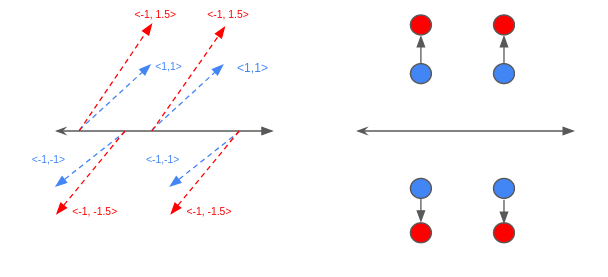
\includegraphics[width=8cm]{scale.png}\\
	\textbf{Figure 4}
\end{center}

\par\noindent If we can imagine every pixel of the image as being the tip of a vector, and apply the transformation described above we will see that the image stretches vertically:

\begin{center}
	
\includegraphics[width=4cm]{cate-original.jpg}
	
\includegraphics[width=4cm]{cate-scaled.jpg}\\
	\textbf{Figure 5}
\end{center}

\subsection {Shearing}
\par \noindent We will now consider the following transformation:
\[
\left(\begin{array}{@{}cc@{}}
	1 & 1.5 \\
	0 & 1\\
\end{array}\right)
\left(\begin{array}{@{}c@{}}
	x \\
	y \\
\end{array}\right)= B
\]

\par \noindent Supposed we provided \(\vec v = <1,1>\) to the transformation, in return we would get \(<2.5,1>\). The diagram below shows the result of transforming a few vectors:

\begin{center}
	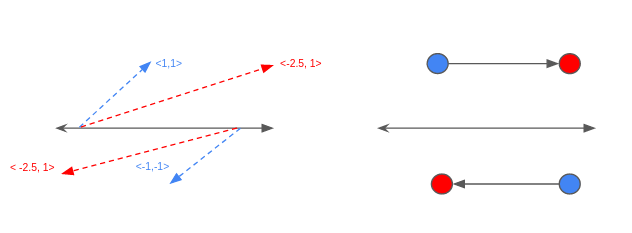
\includegraphics[width=8cm]{shear.png}\\
	\textbf{Figure 6}
\end{center}

\par\noindent If we apply this shear to all the pixels on an image, we would observe the following:

\begin{center}
	
\includegraphics[width=4cm]{cate-original.jpg}
	
\includegraphics[width=5.5cm]{cate-sheared.jpg}\\
	\textbf{Figure 7}
\end{center}

\end{document}	